\subsection{Signal efficiency}\label{sec:WBoson_Analysis_Efficiency}

The \WToMuNu signal efficiency is defined as the probability for a muon with $\pt > 25$~\GeVc and $\abs{\etaMuLAB} < 2.4$, to be reconstructed and pass all the analysis selection criteria. The signal efficiency is obtained from simulation as detailed in \sect{sec:WBoson_Analysis_Efficiency_Simulated} and then corrected using data-to-MC efficiency ratios derived with the tag-and-probe method as explained in \sect{sec:WBoson_Analysis_Efficiency_Corrected}.

\subsubsection{Simulated signal efficiency}\label{sec:WBoson_Analysis_Efficiency_Simulated}

The signal efficiency is estimated using the \WToMuNu simulations since they contain the full history of the signal events, including the generation and reconstruction of the particles. To improve the modelling of the event activity in \RunpPb and the \Wb-boson \pt spectrum, the distributions of the generated \Wb-boson \pt and simulated HF energy are weighed per event as explained in \sect{sec:WBoson_Analysis_Corrections_WeakBosonPTReweighing} and \sect{sec:WBoson_Analysis_Corrections_EventActivityReweighing}, respectively.

A reconstructed muon is considered an offline muon if it satisfies the signal selection requirements. Among the selection criteria, an offline muon is required to satisfy the isolation and identification criteria defined in \sect{sec:WBoson_Analysis_Selection_MuonIdentification}, match the trigger, have $\ptMu~>~25$~\GeVc and be within the CMS detector coverage $|\etaMuLAB|~<~2.4$.

The signal efficiency of the simulated events is computed as the fraction of \textit{generated} muons matched to an \textit{offline} muon around a cone of $\Delta{R} = \sqrt{\Delta{\eta}^{2} + \Delta{\phi}^{2}} < 0.05$.  All generated muons are required to be within the analysis kinematic region ($\ptMu~>~25$~\GeVc and $\abs{\etaLAB}~<~2.4$) and come from a \Wb-boson decay. The signal efficiency of the \pPb and \Pbp \WToMuNu simulations is derived as a function of the generated muon \etaMuLAB, according to:

\begin{equation}
 \epsilon^{\mu^{\pm}}_{\pPb\,(\Pbp)}\left(\etaMuLAB\right) = \left(\frac{N_{\text{off}}^{\mu^{\pm}}\left[\etaMuLAB\right]}{N_{\gen,\pt>25\GeVc}^{\mu^{\pm}}\left[\etaMuLAB\right]}\right)_{\pPb\,(\Pbp)}
 \label{eq:MCTruthEfficiency}
\end{equation}

where $N_{\text{off}}$ and $N_{\gen}$ are the number of offline and generated muons, accordingly. A comparison of the signal efficiencies from the \pPb and \Pbp simulations is shown in \fig{fig:MCTruthComparison}. A good agreement between the two samples is observed.

\begin{figure}[htb!]
 \centering
 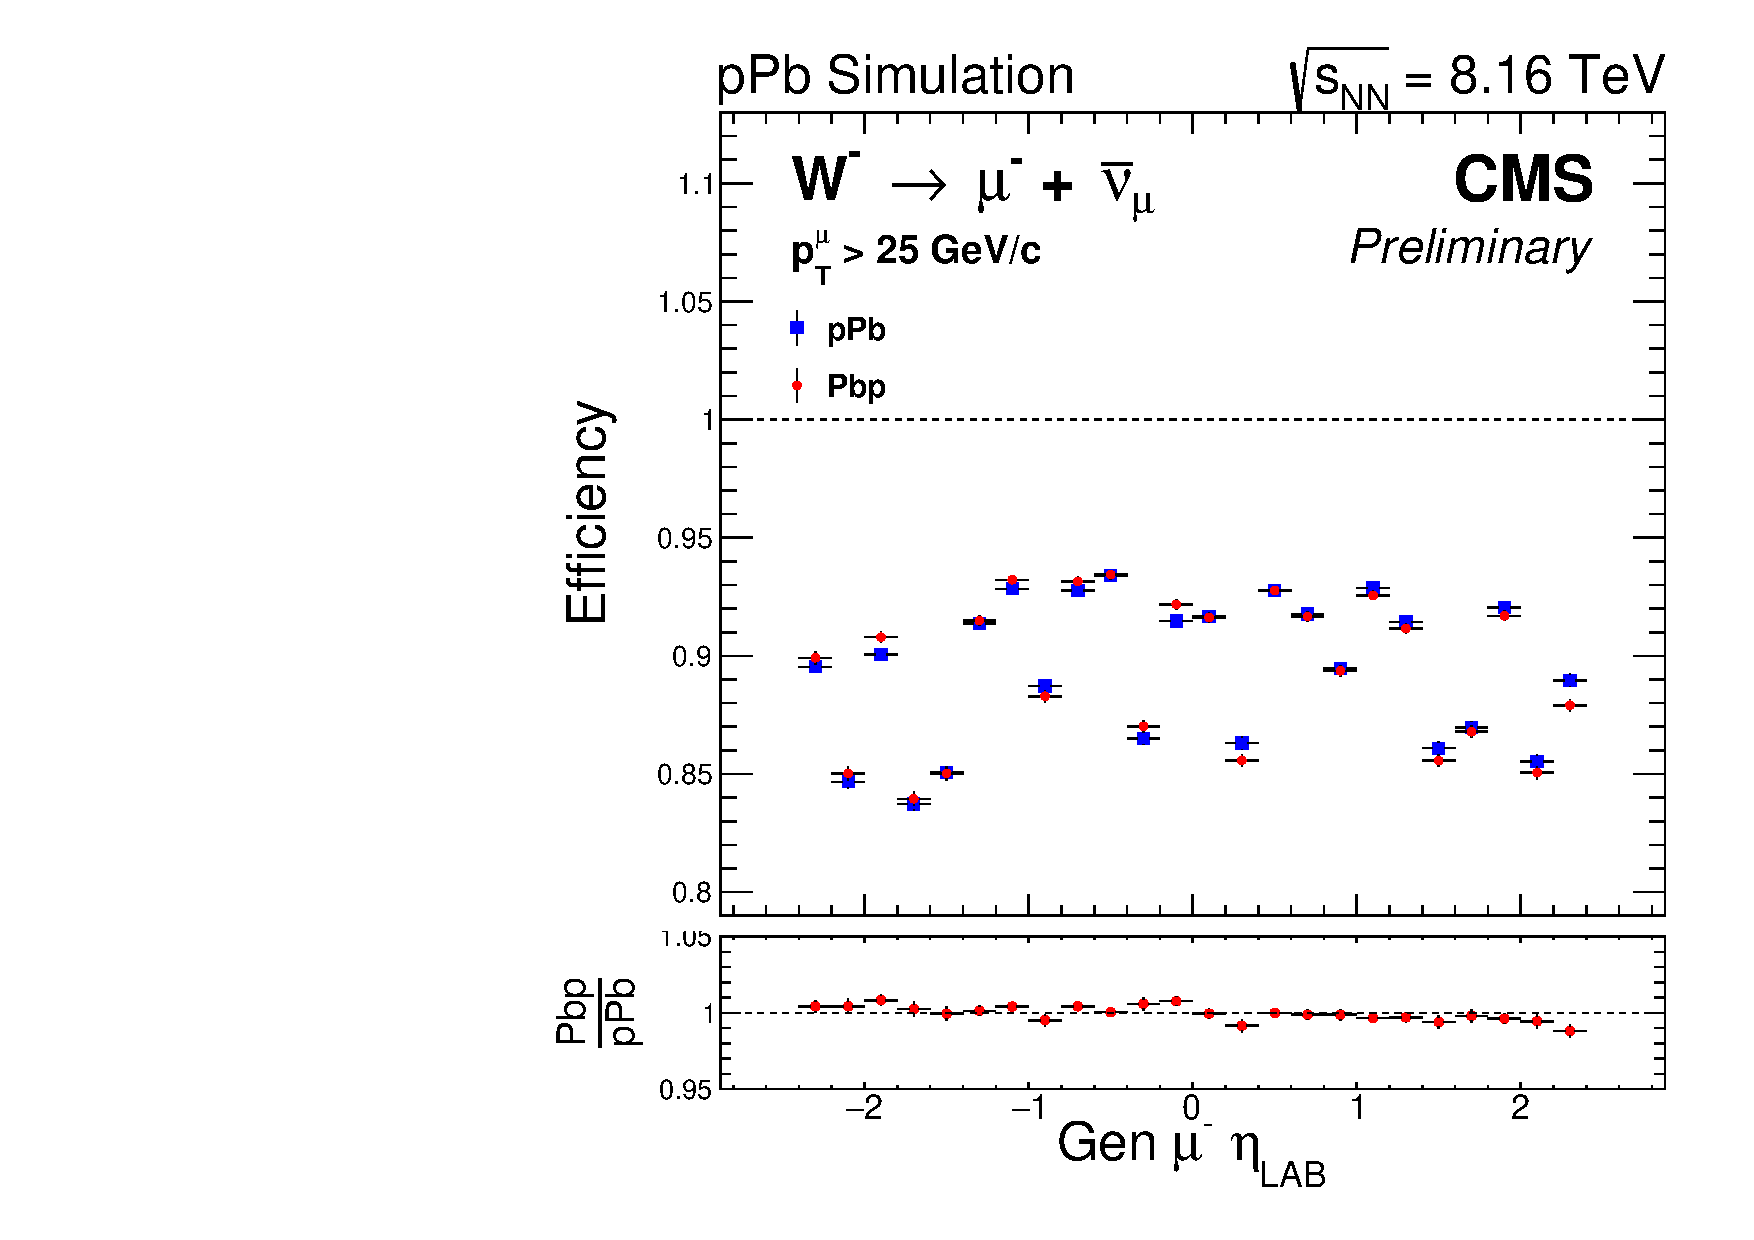
\includegraphics[width=0.45\textwidth]{Figures/WBoson/Analysis/Efficiency/eff1D_Eta_MC_WToMuNu_Minus_Total_HFCorr.pdf}
 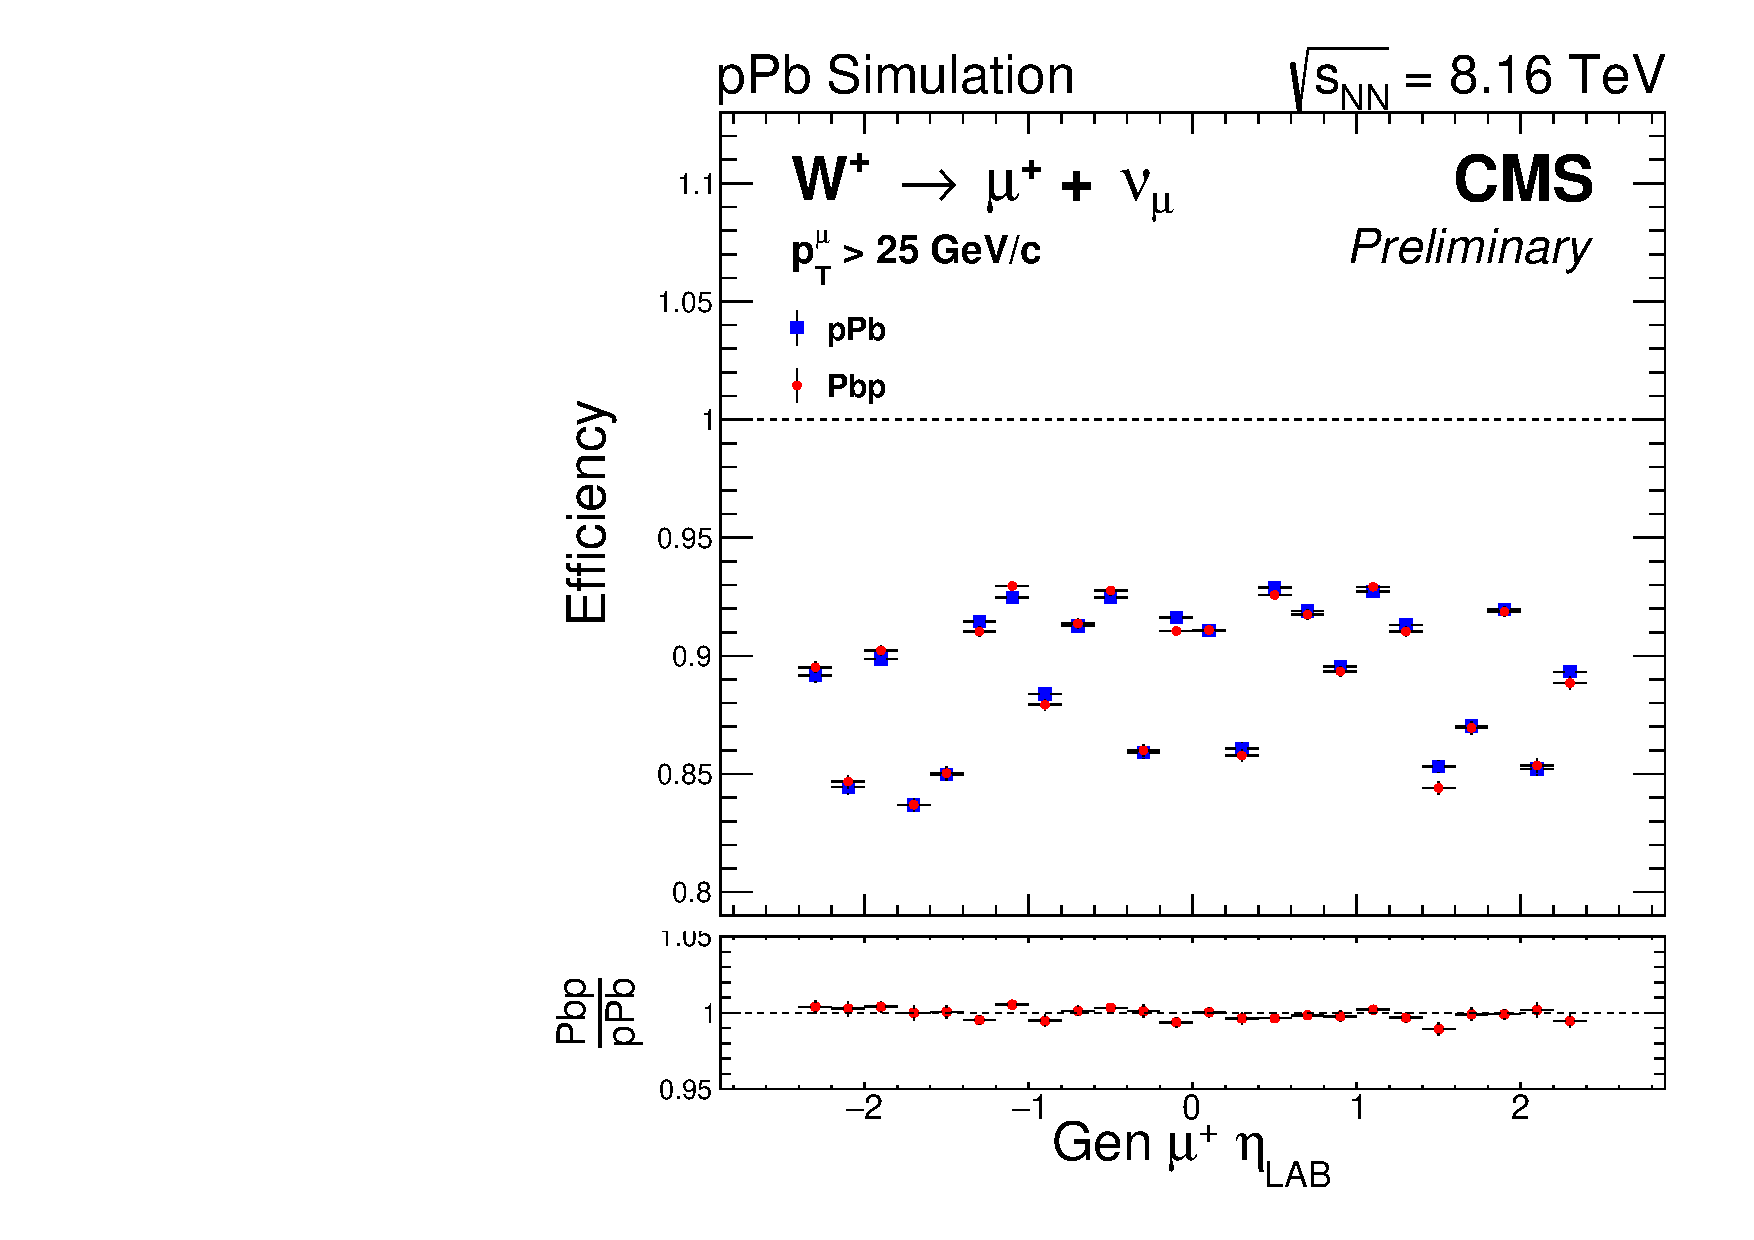
\includegraphics[width=0.45\textwidth]{Figures/WBoson/Analysis/Efficiency/eff1D_Eta_MC_WToMuNu_Plus_Total_HFCorr.pdf}
 \caption{Comparison of the signal efficiency derived from the \pPb and \Pbp \WToMuNu simulations as a function of the generated muon \etaLAB, separated in negative (left) and positive (right) charged muons. The distributions of the simulated HF energy and generated \Wb-boson \pt have been weighed. The bottom panel shows the ratio of \Pbp over \pPb signal efficiencies.}
 \label{fig:MCTruthComparison}
\end{figure}

The signal efficiencies extracted from the \pPb and \Pbp \WToMuNu simulations are then combined in the centre-of-mass frame, and the final simulated signal efficiency $\epsilon^{\mu^{\pm}}_{\MC}$ is obtained as:

\begin{equation}
 \epsilon^{\mu^{\pm}}_{\MC}\left(\etaMuCM\right) = \frac{\Lumi_{\pPb}\cdot\epsilon^{\mu^{\pm}}_{\pPb}\left(\etaMuCM\right) + \Lumi_{\Pbp}\cdot\epsilon^{\mu^{\pm}}_{\Pbp}\left(\etaMuCM\right)}{\Lumi_{\pPb} + \Lumi_{\Pbp}}
 \label{eq:MCEfficiencyPA}
\end{equation}

where $\Lumi_{\pPb}$ and $\Lumi_{\Pbp}$ are the recorded integrated luminosity of each \RunpPb run. The results of the \WToMuNu efficiency, extracted from the simulations, are shown in \fig{fig:MCTruthEfficiency}.

\begin{figure}[htb!]
 \centering
 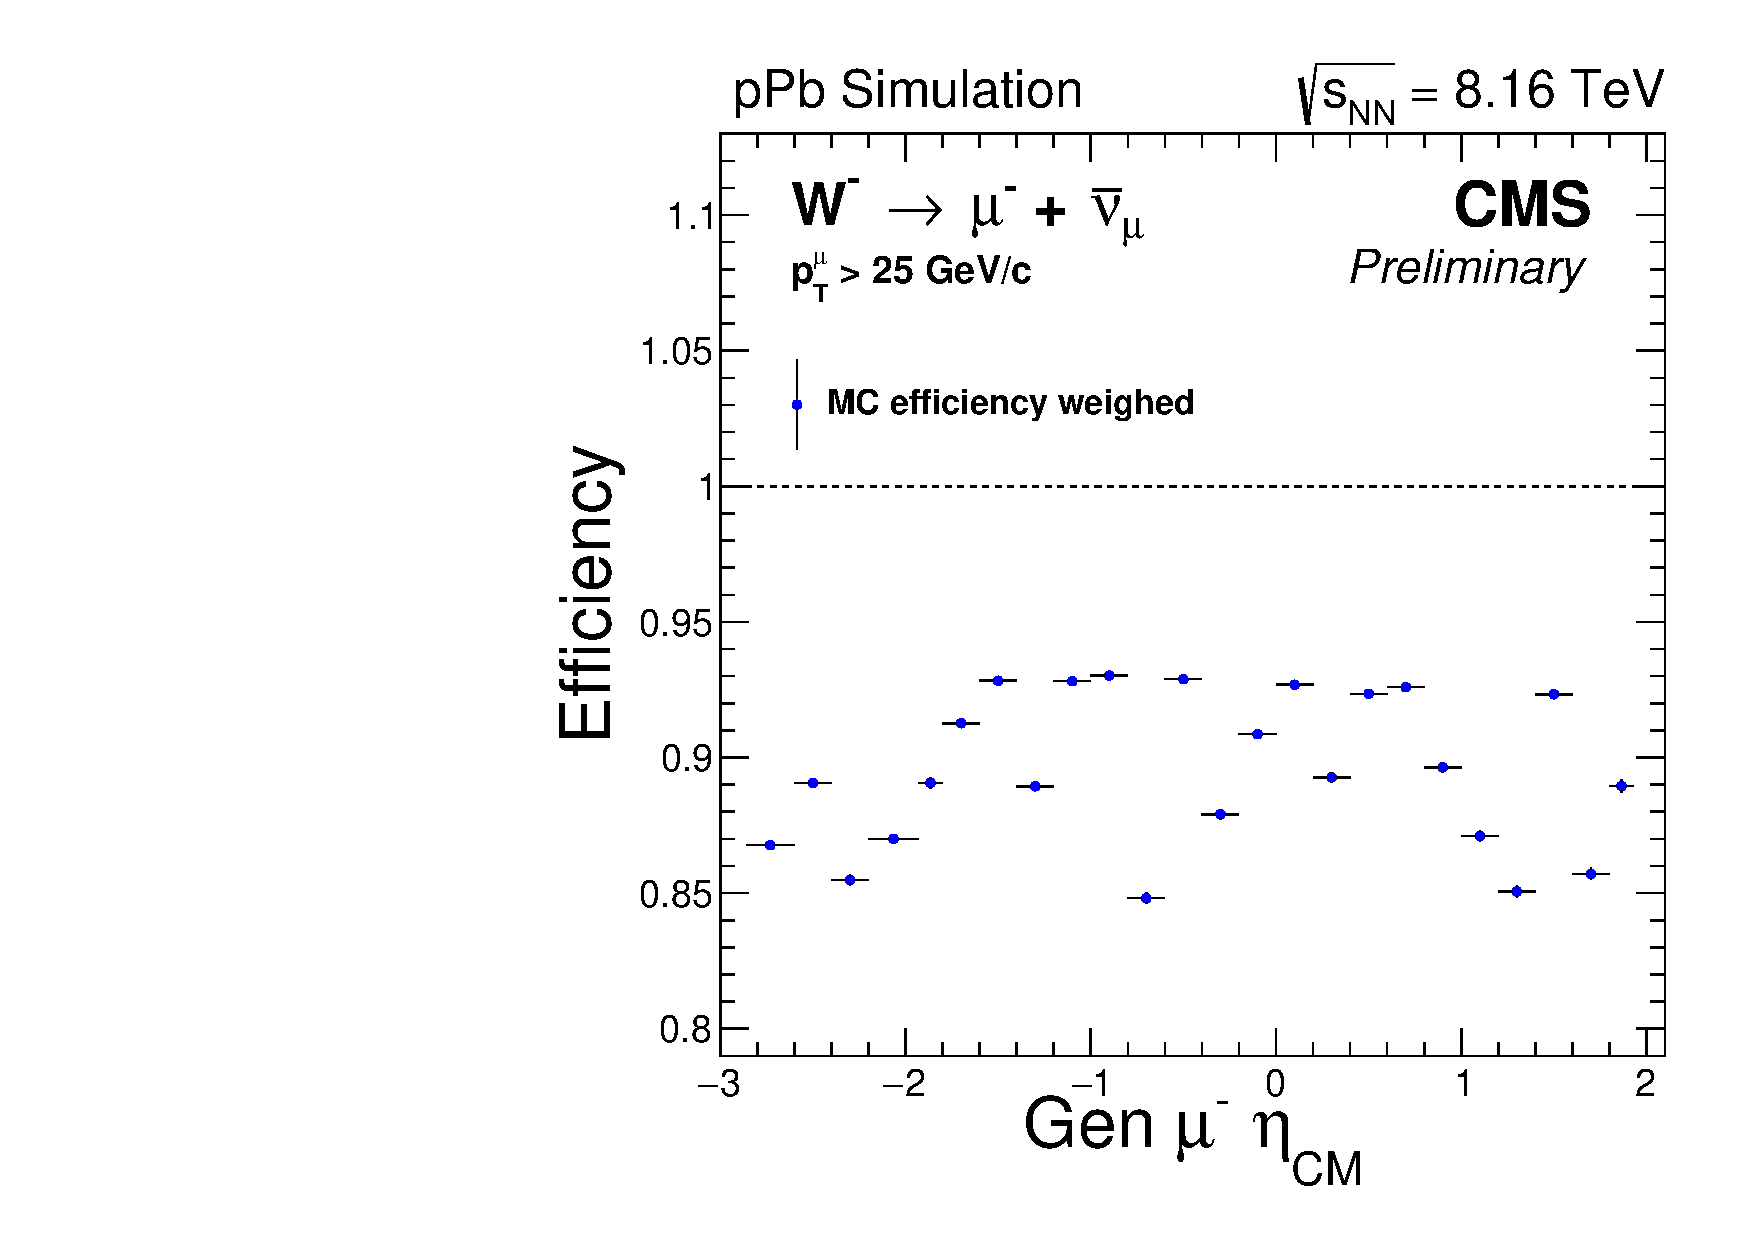
\includegraphics[width=0.45\textwidth]{Figures/WBoson/Analysis/Efficiency/eff1D_EtaCM_MC_WToMuNu_PA_Minus_Total_HFCorrOnly}
 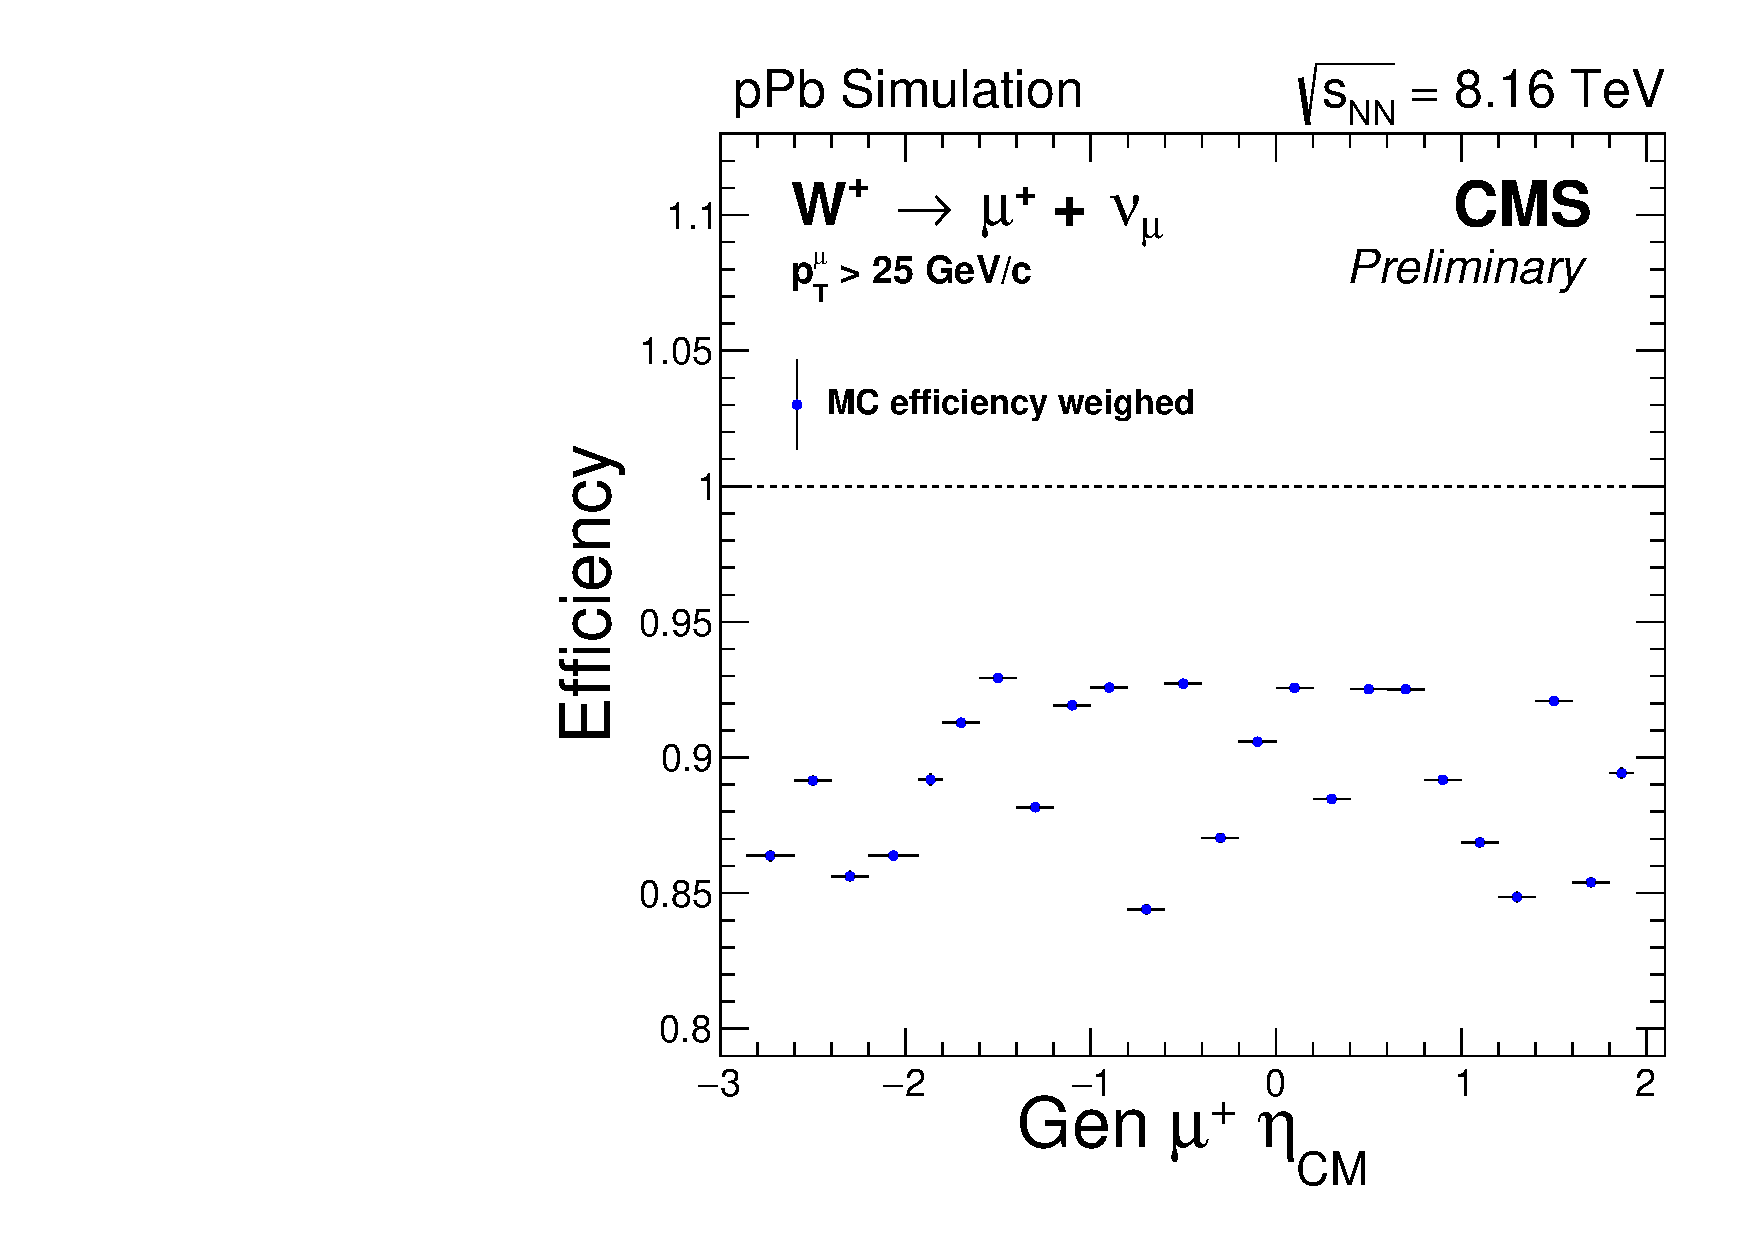
\includegraphics[width=0.45\textwidth]{Figures/WBoson/Analysis/Efficiency/eff1D_EtaCM_MC_WToMuNu_PA_Plus_Total_HFCorrOnly}
 \caption{Simulated signal efficiency derived from the \WToMuNu NLO simulations as a function of the generated muon \etaCM, separated in negative (left) and positive (right) charged muons. The distributions of the simulated HF energy and generated \Wb-boson \pt have been weighed.}
 \label{fig:MCTruthEfficiency}
\end{figure}

\subsubsection{Corrected signal efficiency}\label{sec:WBoson_Analysis_Efficiency_Corrected}

The simulation of the CMS detector is very precise but still far from fully describing all the detector conditions observed in real data. In order to compensate for the imperfections in the simulation, a set of data-to-MC corrections provided by the CMS heavy-ion (HIN) group are used to improve the estimation of the signal efficiency. These corrections are derived from the ratio of efficiencies measured in data and simulation using the tag-and-probe (\tnp) method.

The tag-and-probe method is a data-driven technique widely used to compute efficiencies of physical objects, such as muons, produced from the decay of known mass resonances (e.g. \Z bosons). One advantage of the \tnp method is that it can be applied to data and simulation, allowing to assess the possible  differences between the data and simulated muon efficiencies. The \tnp analysis performed in \RunpPb collisions by the CMS HIN group is documented in the internal analysis note~\cite{Muon_TnP_pPb}.

\paragraph{Definition of the tag-and-probe efficiencies.} To study the different elements that enter in the reconstruction and selection of muons, the total muon efficiency is factorised in five different components, according to:

\begin{equation}
 \epsilon^{\mu} = \epsilon_{\text{STA}}\cdot\epsilon_{\text{TRK}}\cdot\epsilon_{\text{ID}}\cdot\epsilon_{\text{Trig}}\cdot\epsilon_{\text{Iso}}
\end{equation}

where each efficiency component is defined relative to the previous one, as described below:

\begin{itemize}
 \item $\epsilon_{\text{STA}}$ : represents the standalone-muon (STA) reconstruction efficiency. It is probed by tracker tracks and is derived by matching the probe to a standalone muon.
 \item $\epsilon_{\text{trk}}$ : represents the global muon tracking efficiency. It is probed by standalone muons and is derived by matching the probe to a global muon.
 \item $\epsilon_{\text{ID}}$ : represents the muon identification efficiency. It is probed by global muons and is determined by requiring that the probe satisfies the tight identification criteria defined in \sect{sec:WBoson_Analysis_Selection_MuonIdentification}.
 \item $\epsilon_{\text{trig}}$ : represents the muon trigger efficiency. It is probed by global muons passing the identification criteria, and is determined by requiring that the probe is matched to the muon trigger.
 \item $\epsilon_{\text{iso}}$ : represents the muon isolation efficiency. It is probed by global muons passing the identification criteria and matched to the trigger, and it is computed by requiring that the probe pass the muon isolation requirement ($\iso < 0.15$).
\end{itemize}


\paragraph{Extraction of the tag-and-probe efficiencies.} For high-\pt muons ($\pt > 15$~\GeVc), the dimuon decay of \Z bosons is used to create a clean sample. In each event, a high-quality muon, called the \textit{tag}, is combined with the \textit{probe} of the efficiency being measured, to form a tag-probe pair within the \Z-boson mass window. The tag and the probe are required to have $\pt > 15$~\GeVc and be inside the acceptance of CMS ($|\etaLAB| < 2.4$). In addition, the tag is also required to satisfy the muon isolation and identification criteria, and be matched to the trigger.

The tag-probe pairs are separated into two samples depending on whether the probe pass the selection criteria under study. The efficiency is then determined by performing a simultaneous unbinned maximum likelihood fit to the tag-probe invariant mass distribution ($m_{\text{TP}}$) for failing and passing probes. The \ZToMuMu signal distributions are parametrised with a Voigt profile~\cite{Voigt} and the background distributions with an  exponential. The same procedure is performed for all efficiencies measured in data and simulation.

As an example, the fits to the tag-probe invariant mass distribution for passing and failing probes, used to measure the STA reconstruction efficiency, are shown in \fig{fig:TnPFits}.

\begin{figure}[htb!]
 \centering
 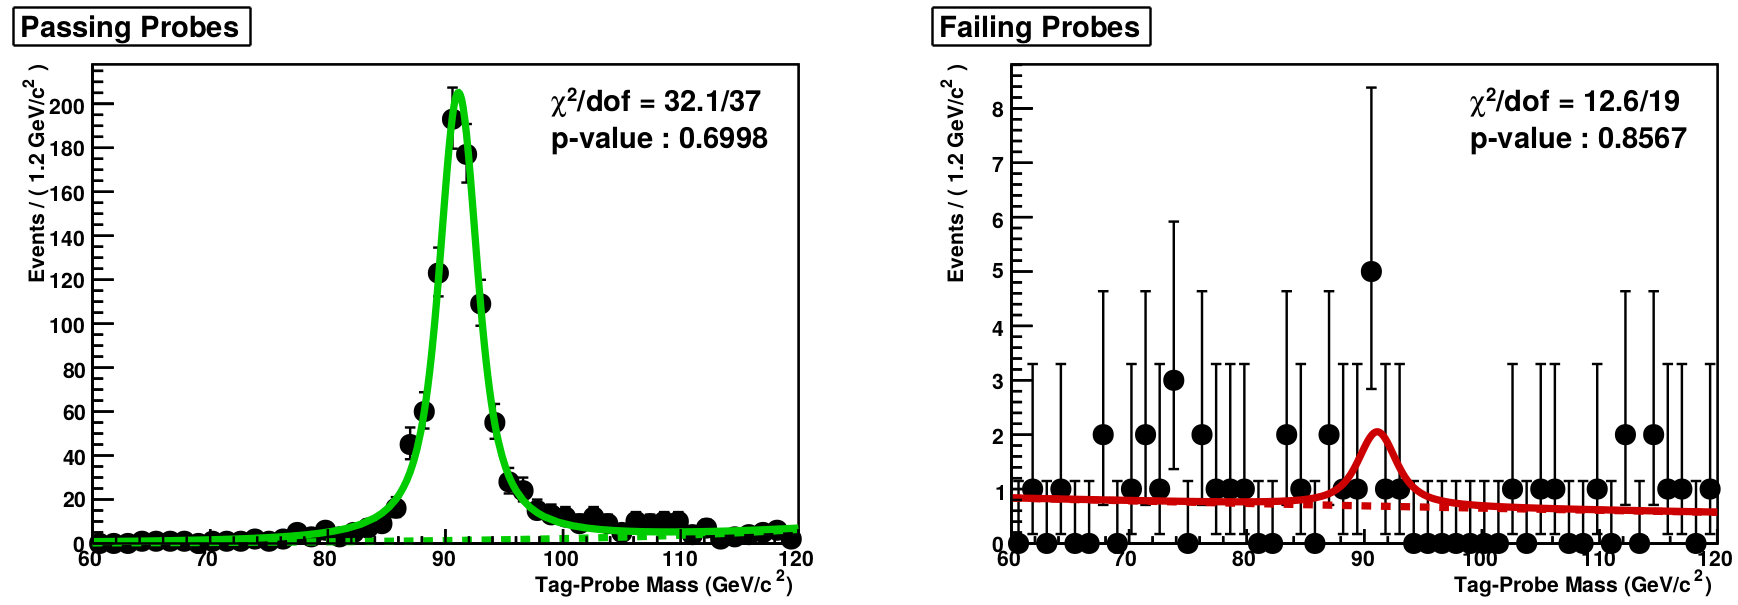
\includegraphics[width=1.0\textwidth]{Figures/WBoson/Analysis/Efficiency/TnP/TnPFit.png}
 \caption{Fits to the tag-probe invariant mass distribution for passing (left) and failing (right) probes, used to measure the STA reconstruction efficiency. The results correspond to the probe kinematic region: $\abs{\etaLAB}<2.4$ and $50 < \pt < 80$~\GeVc. Figures taken from the internal analysis note~\cite{Muon_TnP_pPb}.}
 \label{fig:TnPFits}
\end{figure}


\paragraph{Results of the tag-and-probe efficiencies.} The STA reconstruction $\epsilon_{\text{STA}}$ and global muon tracking $\epsilon_{\text{trk}}$ efficiencies are found to agree between data and simulation within an uncertainty of $0.6\%$ and $<0.1\%$, respectively, and no correction is required for the simulated \WToMuNu efficiency.

In the case of the muon identification $\epsilon_{\text{ID}}$ and isolation $\epsilon_{\text{iso}}$ efficiencies, the results obtained from simulation are observed to disagree with those from data, as shown in  \fig{fig:TnPEfficiencyIDIso}. As a result, the efficiencies measured in data and simulation, as a function of the probed \pt, are fitted with: a linear function ($f_{\text{ID}}(\pt) = a\cdot\pt + b$) for muon identification and a displaced error function ($f_{\text{iso}}(\pt) = a\cdot\text{Erf}[(\pt - c)/b] + d$) for  muon isolation. The fits to the efficiencies are performed in three regions of probe \etaLAB, corresponding to: $\abs{\etaMuLAB} < 1.2$,   $1.2 < \abs{\etaMuLAB} < 2.1$ and  $2.1 < \abs{\etaMuLAB} < 2.4$. The ratios of the fitted functions extracted from the data and simulation efficiencies, for muon identification  ($w_{\text{ID}} = f^{\data}_{\text{ID}}\big/f^{\MC}_{\text{ID}}$) and for muon isolation ($w_{\text{iso}} = f^{\data}_{\text{iso}}\big/f^{\MC}_{\text{iso}}$), are used as \tnp corrections for the simulated \WToMuNu efficiency.

\begin{figure}[htb!]
 \centering
 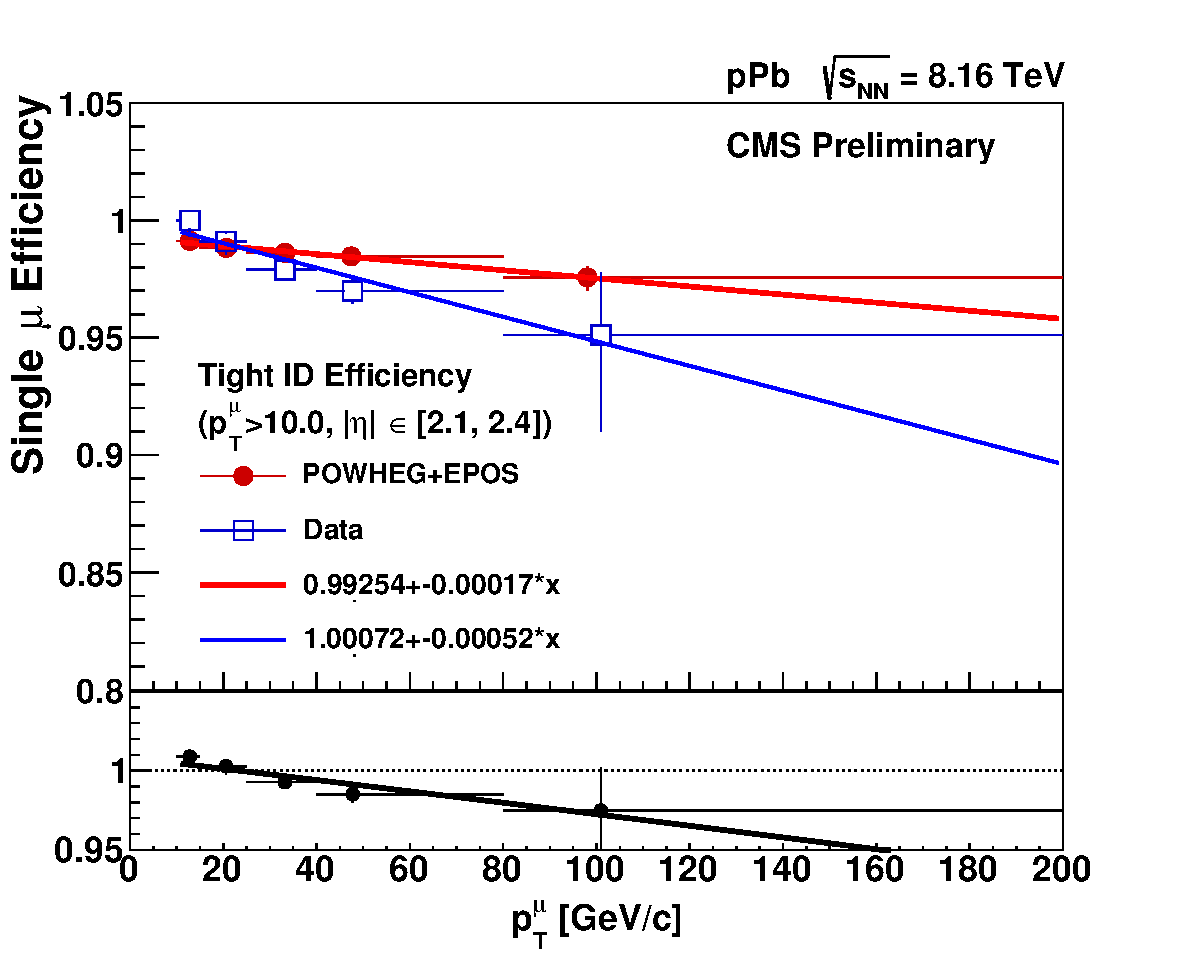
\includegraphics[width=0.49\textwidth]{Figures/WBoson/Analysis/Efficiency/TnP/tpTreeSF7_pPb_RD_MC_PT.pdf}
 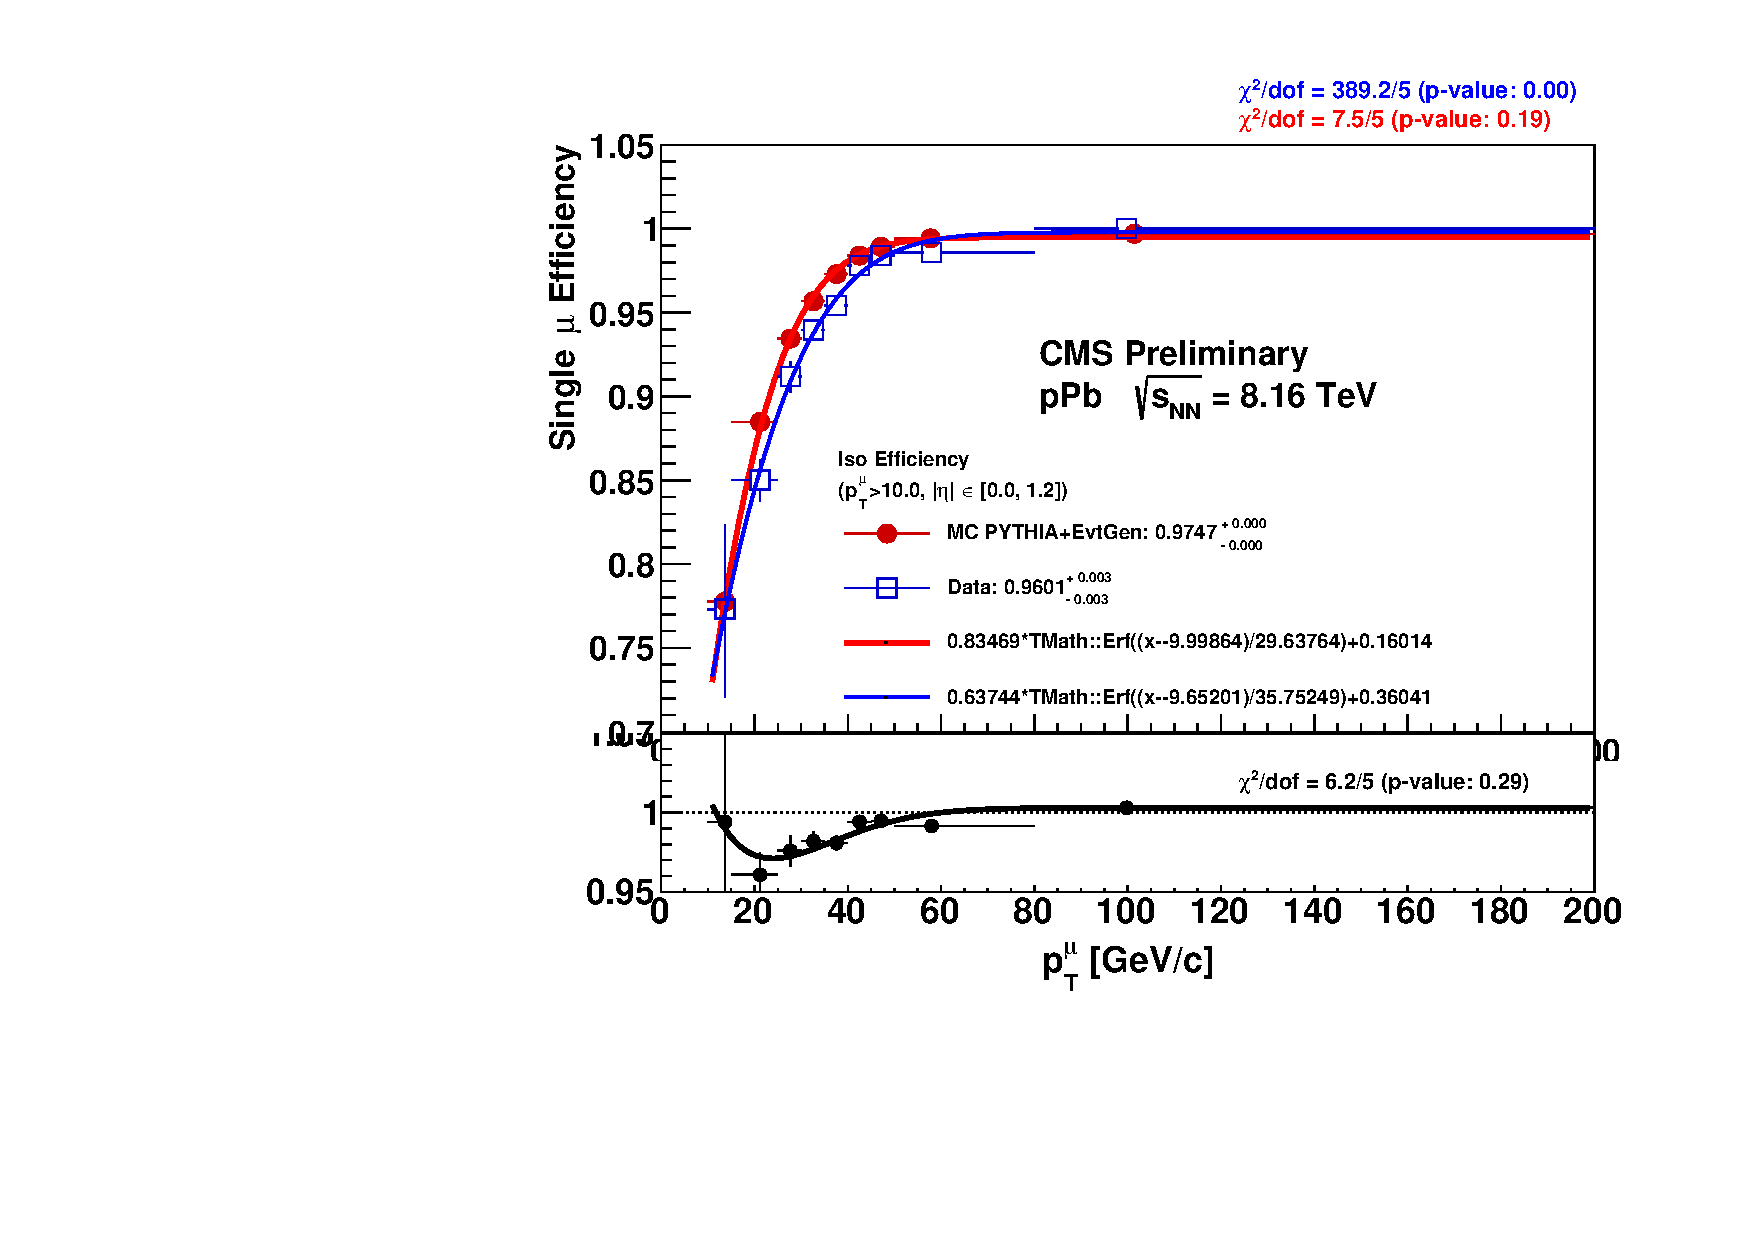
\includegraphics[width=0.49\textwidth]{Figures/WBoson/Analysis/Efficiency/TnP/tpTreeSF3_pPb_RD_MC_PT.pdf}
 \caption{Muon identification (left) and isolation (right) efficiencies extracted from data (blue) and simulation (red) using the \tnp method, as a function of the probe \pt. The bottom panels show the data-to-simulation efficiency ratio. The results of the fits to the efficiencies are also shown. Figures taken from the internal analysis note~\cite{Muon_TnP_pPb}.}
 \label{fig:TnPEfficiencyIDIso}
\end{figure}

The muon trigger efficiency $\epsilon_{\text{trig}}$ extracted from the simulation is seen to disagree with the results from data as a function of the probe \etaLAB, as presented in \fig{fig:TnPEfficiencyTrigger}. In this case, the ratio of the measured efficiency extracted from data and simulation ($w_{\text{trig}} = \epsilon^{\data}_{\text{ID}}\big/\epsilon^{\MC}_{\text{ID}}$), in each bin of probe \etaLAB, is used to correct the simulated \WToMuNu efficiency.

\begin{figure}[htb!]
 \centering
 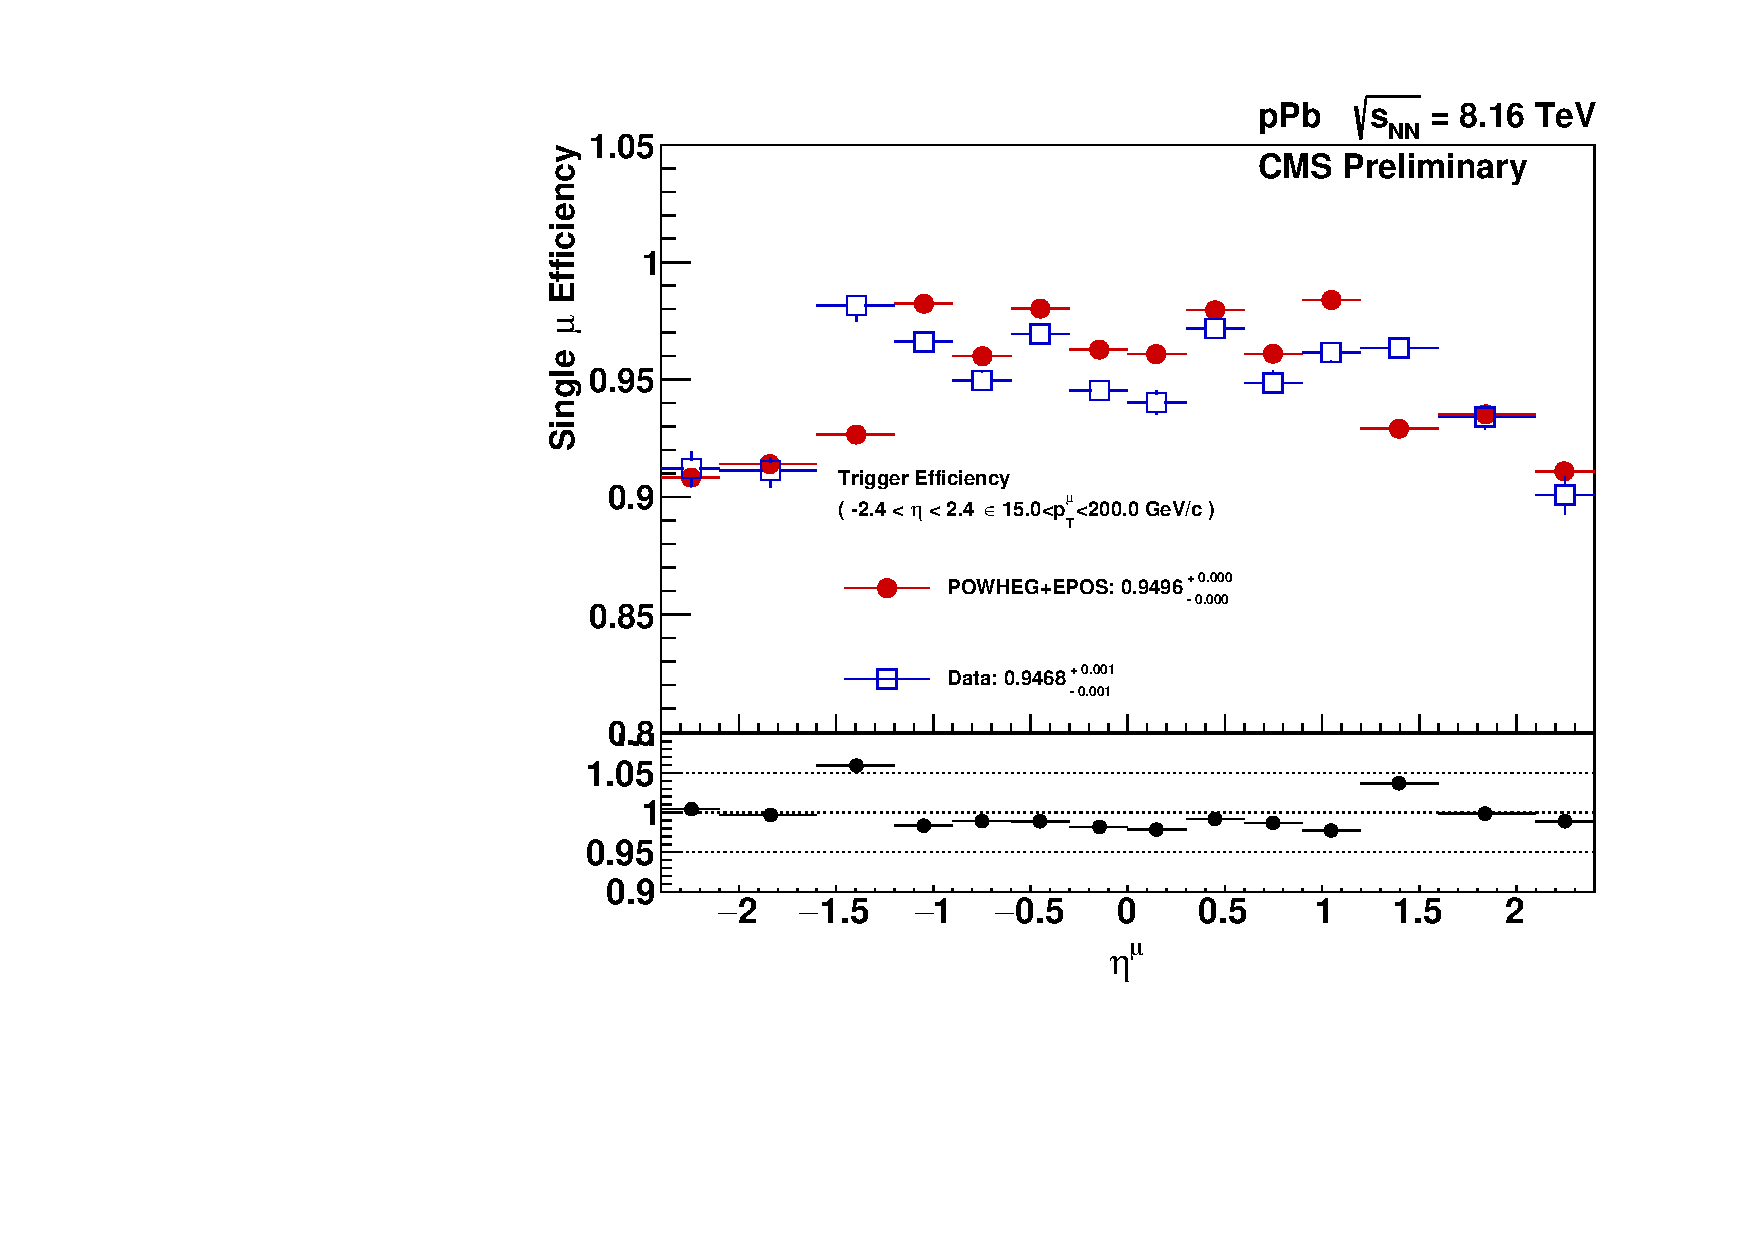
\includegraphics[width=0.49\textwidth]{Figures/WBoson/Analysis/Efficiency/TnP/tpTreeEff0_pPb_RD_MC_Eta.pdf}
 \caption{Muon trigger efficiency extracted from data (blue) and simulation (red) using the \tnp method, as a function of the probe \etaLAB. The bottom panel shows the data-to-simulation efficiency ratio. Figure taken from the internal analysis note~\cite{Muon_TnP_pPb}.}
 \label{fig:TnPEfficiencyTrigger}
\end{figure}

\paragraph{Correction of the signal efficiency.} The simulated signal efficiency is recomputed by weighing the offline muon yield per event using the \tnp corrections provided by the CMS HIN group, for muon identification $w_{\text{ID}}$, trigger $w_{\text{trig}}$ and isolation $w_{\text{iso}}$, according to:

\begin{equation}
 \epsilon^{\mu^{\pm}}_{\corr} = \frac{\left[\sum\limits_{i=1}^{N_{\text{off}}^{\mu^{\pm}}} w_{\text{ID}}\left(\ptMu, \abs{\etaMuLAB}\right) \cdot w_{\text{trig}}\left(\etaLAB\right) \cdot w_{\text{iso}}\left(\ptMu, \abs{\etaMuLAB}\right)\right]}{N_{\gen,\pt>25\GeVc}^{\mu^{\pm}}}
\end{equation}

where the \tnp corrections are evaluated as a function of the offline muon \pt and \etaLAB in each event, and the sum is performed over the simulated signal events.

\paragraph{Uncertainties of the tag-and-probe corrections.} The uncertainties associated to the \tnp corrections are driven by the larger background and lower statistics present in data. As a result, only the uncertainties associated to the data efficiencies are propagated to the \tnp corrections, while the simulation efficiencies are fixed. The statistical and systematic components of the \tnp correction uncertainties are estimated by performing the following set of variations:

\begin{itemize}

 \item (A) Statistical uncertainty for muon ID and isolation: estimated by generating a hundred sets of \tnp corrections using pseudo-experiments. For each pseudo-experiment, the data efficiency points are randomly varied based on a Gaussian distribution of width equal to the statistical uncertainty of the efficiency points.

 \item (B) Statistical uncertainty for muon trigger: estimated with two sets of \tnp corrections, determined by varying the data efficiency points up and down according to their statistical uncertainty.

 \item (C) Systematic uncertainty of the efficiency extraction: derived by refitting the tag-probe invariant mass distributions after varying the signal and background functional forms, and by extending the range of the \Z-boson mass window. These uncertainties are then propagated to the \tnp corrections by varying the data efficiency points up and down by one standard deviation, producing two sets of \tnp corrections.

 \item (D) Systematic uncertainty of the efficiency parametrisation for muon ID and isolation: estimated by using the ratio of the efficiency points from data and simulation ($w = \epsilon^{\data}\big/\epsilon^{\MC}$), instead of the fitted efficiency curves.

\end{itemize}

In addition, an uncertainty of $0.34\%$ is included to account for the impact of the different level of event activity present in data and simulation. This is derived by comparing the simulated muon isolation efficiency  before and after applying the HF energy weighing. Moreover, the uncertainty of $0.6\%$ is also added to account for possible mismodelling of the STA reconstruction efficiency, determined from the level of agreement between data and simulation.

The uncertainties of the \tnp corrections are propagated to the signal efficiency in two ways:

\begin{itemize}
 \item For the hundred \tnp corrections described in (A): the signal efficiency is recomputed with each of the \tnp corrections and the RMS of the hundred signal efficiencies obtained is then taken as the uncertainty on the signal efficiency.
 \item For the up and down variations used in (B), (C) and (D): the uncertainty on the signal efficiency is determined from the largest difference between applying the up or down varied \tnp corrections and the nominal one.

\end{itemize}

The total uncertainty on the signal efficiency due to \tnp corrections, is obtained by summing in quadrature the uncertainties from (A), (B), (C) and (D). The additional relative uncertainties of 0.34\% and 0.6\% are also included.


\paragraph{Results of the signal efficiency correction.} The corrected signal efficiency is shown in \fig{fig:CorrEfficiency}, including the  uncertainties due to \tnp correction. 

\begin{figure}[htb!]
 \centering
 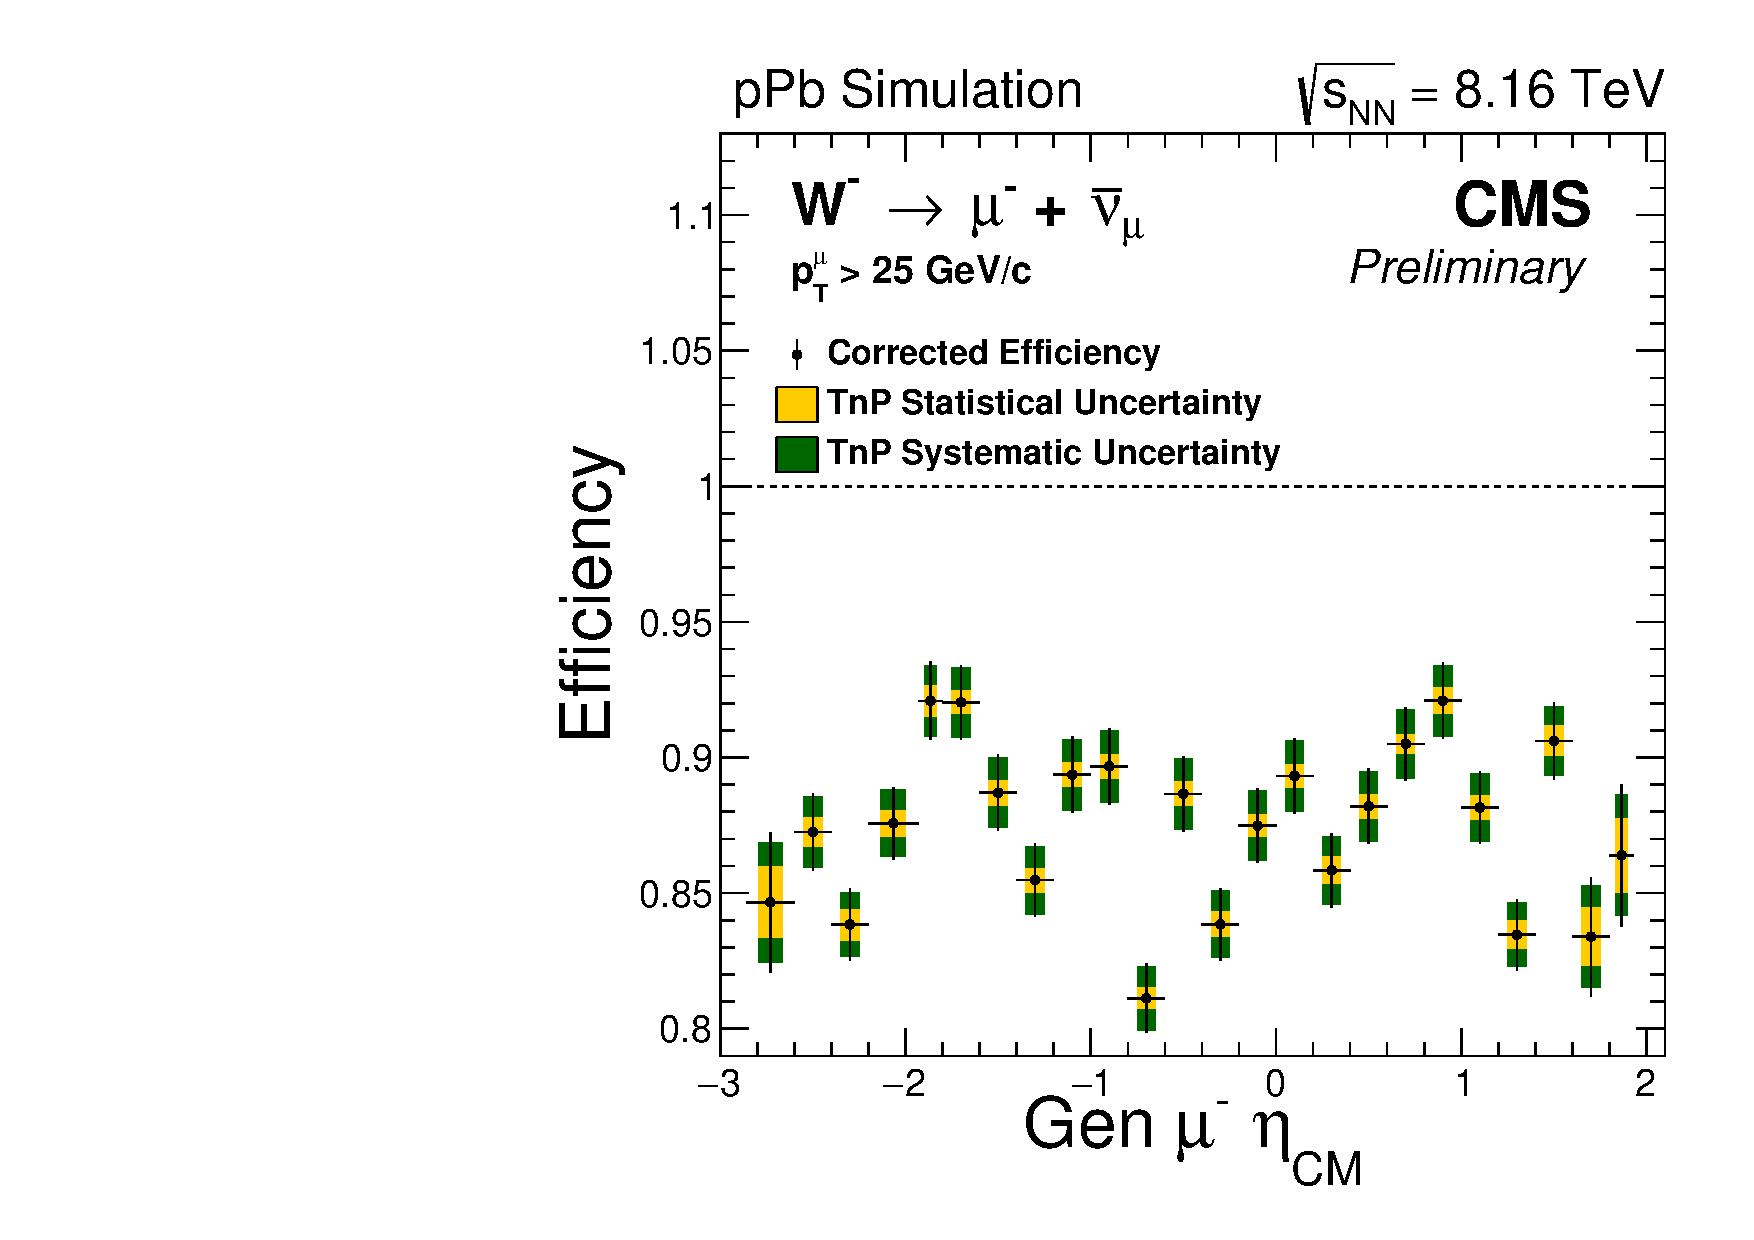
\includegraphics[width=0.45\textwidth]{Figures/WBoson/Analysis/Efficiency/eff1D_EtaCM_MC_WToMuNu_PA_Minus_Total_TnP_Nominal}
 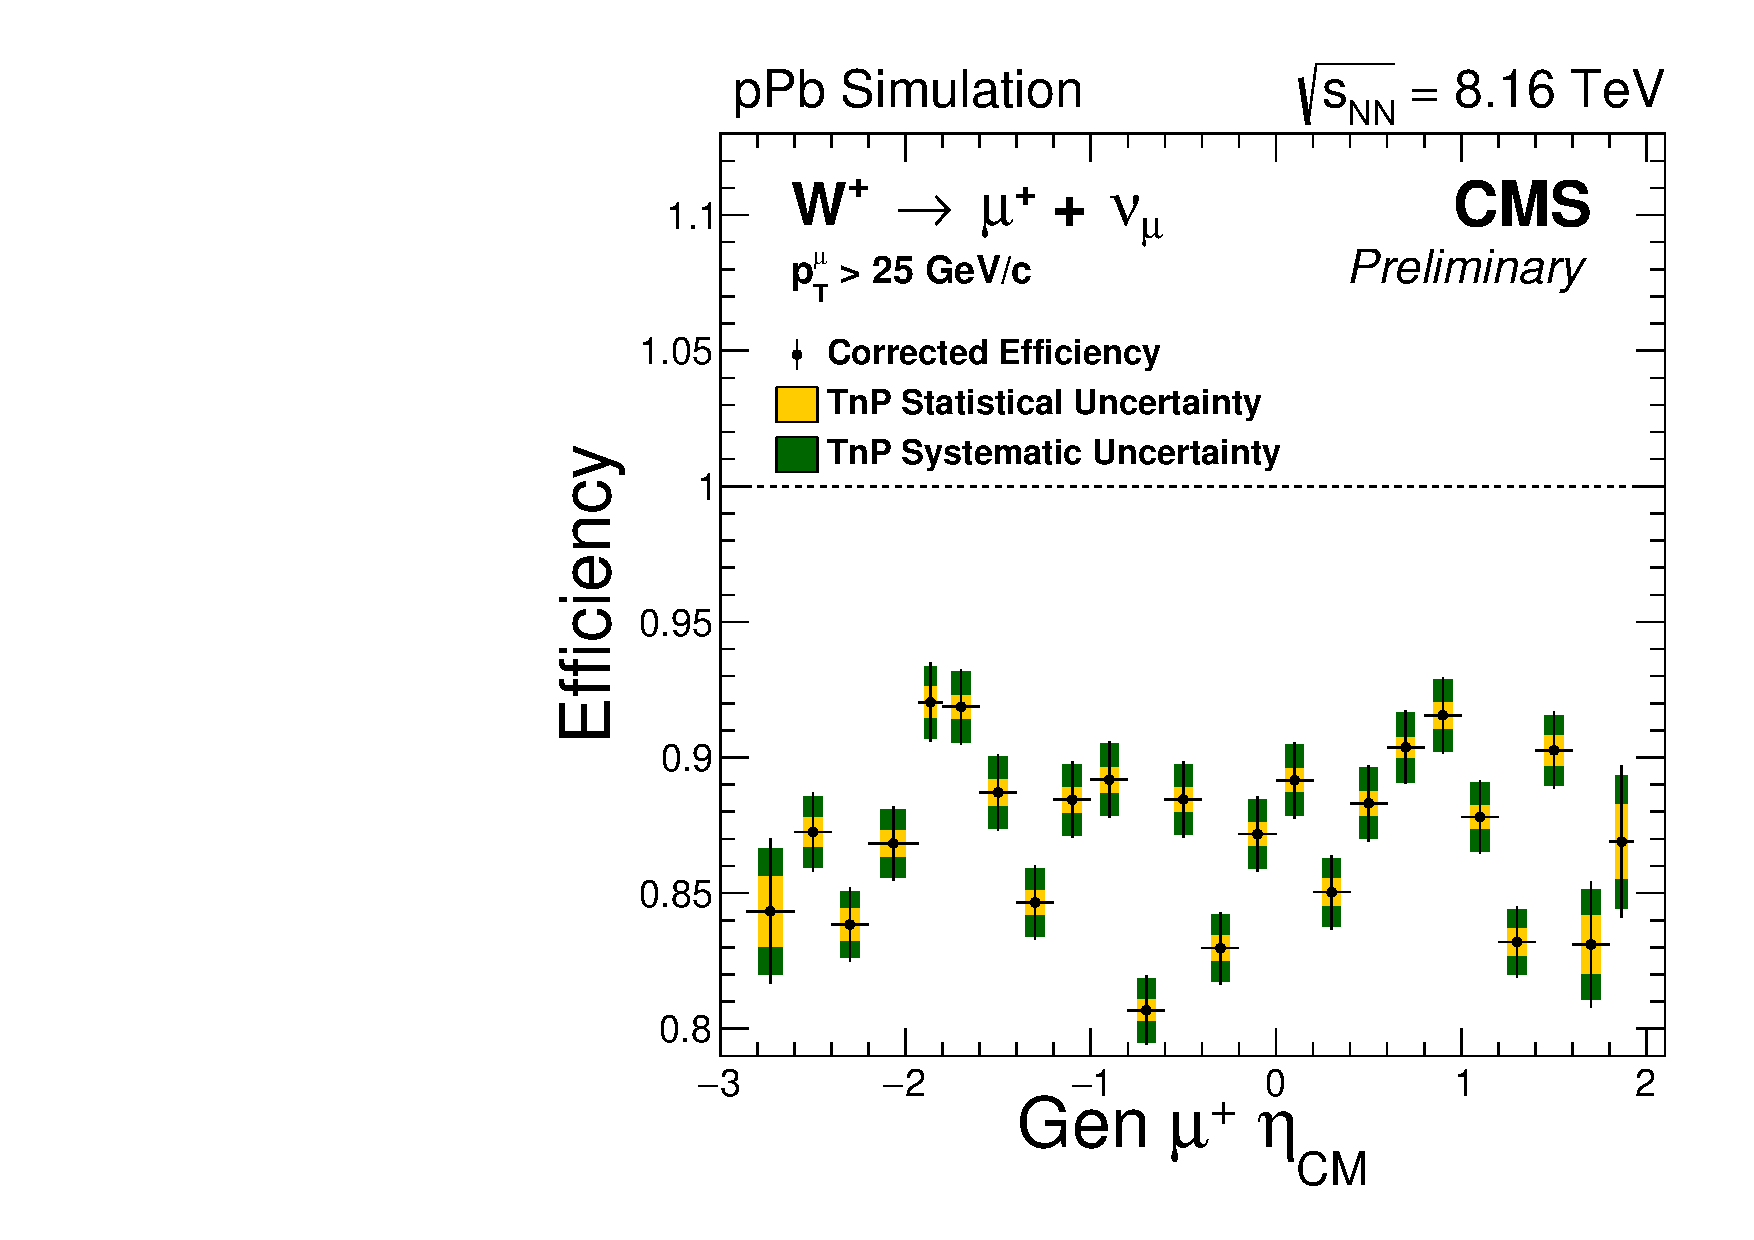
\includegraphics[width=0.45\textwidth]{Figures/WBoson/Analysis/Efficiency/eff1D_EtaCM_MC_WToMuNu_PA_Plus_Total_TnP_Nominal}
 \caption{Corrected signal efficiency as a function of the generated muon \etaCM, separated in negative (left) and positive (right) charged muons. The yellow and green boxes represents the uncertainty on the signal efficiency due to the \tnp statistics and systematics, respectively.}
 \label{fig:CorrEfficiency}
\end{figure}

The relative difference between the corrected and the simulated signal efficiencies ($(\epsilon_{\corr}-\epsilon_{\MC})\big/\epsilon_{\MC}$), is presented in \tab{tab:compEfficiency_WToMu_PA} as a function of the generated \etaCM. The largest variation due to the \tnp corrections is found to be $4.7\%$.

\begin{table}[htb!]
  \centering
  %\renewcommand{\arraystretch}{1.5}
  \begin{tabular}{|c|*2c|}
    \hline
    $\etaMuCM$ Range & $\mu^{-}$ $\frac{\epsilon_{\corr}-\epsilon_{\MC}}{\epsilon_{\MC}}$ [\%] & $\mu^{+}$ $\frac{\epsilon_{\corr} - \epsilon_{\MC}}{\epsilon_{\MC}}$ [\%]\\
    \hline\hline
    $-$2.86 , $-$2.60 & -2.4 & -2.4\\
    \hline
    $-$2.60 , $-$2.40 & -2.0 & -2.1\\
    \hline
    $-$2.40 , $-$2.20 & -1.9 & -2.1\\
    \hline
    $-$2.20 , $-$1.93 & 0.7 & 0.5\\
    \hline
    $-$1.93 , $-$1.80 & 3.4 & 3.2\\
    \hline
    $-$1.80 , $-$1.60 & 0.8 & 0.6\\
    \hline
    $-$1.60 , $-$1.40 & -4.4 & -4.5\\
    \hline
    $-$1.40 , $-$1.20 & -3.9 & -4.0\\
    \hline
    $-$1.20 , $-$1.00 & -3.7 & -3.8\\
    \hline
    $-$1.00 , $-$0.80 & -3.6 & -3.7\\
    \hline
    $-$0.80 , $-$0.60 & -4.4 & -4.4\\
    \hline
    $-$0.60 , $-$0.40 & -4.6 & -4.6\\
    \hline
    $-$0.40 , $-$0.20 & -4.6 & -4.7\\
    \hline
    $-$0.20 , $+$0.00 & -3.7 & -3.8\\
    \hline
    $+$0.00 , $+$0.20 & -3.6 & -3.7\\
    \hline
    $+$0.20 , $+$0.40 & -3.8 & -3.9\\
    \hline
    $+$0.40 , $+$0.60 & -4.5 & -4.6\\
    \hline
    $+$0.60 , $+$0.80 & -2.3 & -2.3\\
    \hline
    $+$0.80 , $+$1.00 & 2.7 & 2.7\\
    \hline
    $+$1.00 , $+$1.20 & 1.2 & 1.1\\
    \hline
    $+$1.20 , $+$1.40 & -1.9 & -2.0\\
    \hline
    $+$1.40 , $+$1.60 & -1.9 & -2.0\\
    \hline
    $+$1.60 , $+$1.80 & -2.7 & -2.7\\
    \hline
    $+$1.80 , $+$1.93 & -2.9 & -2.8\\
    \hline
  \end{tabular}
  \caption{Relative difference between the corrected and simulated signal efficiencies as a function of the generated muon $\eta_{CM}$, separated in negative and positive charged muons.}
  \label{tab:compEfficiency_WToMu_PA}
\end{table}





% END OF SUBSECTION
